\documentclass[times, 11pt, a4paper]{article}

\usepackage{tabularx}
\usepackage{multirow}
\usepackage[para]{threeparttable}
\usepackage{epsfig}
\usepackage{epstopdf}
\usepackage{tipa}
\usepackage{amsmath}
\usepackage{mdwmath}
\usepackage{mdwtab}
\usepackage{url}
\usepackage{float}
%\usepackage{llncsdoc}
\usepackage[top=1.5in, bottom=1.5in, left=1.2in,right=1in]{geometry}
\usepackage{graphicx}
\usepackage{epstopdf}
\usepackage{verbatim}
\usepackage{enumitem}
\setcounter{secnumdepth}{3}
\setlist{nolistsep}
\linespread{1.25}
\textheight 8.8in
\textwidth 6.2in
\begin{document}
%\begin{frontmatter}


\title{\fontsize{16pt}{19.2pt}\selectfont\bf{ Spatio-temporal Mobility Summary of Individuals }}
\date{}
%\DeclareGraphicsExtensions{.pdf,.jpg,.bmp,.gif,.eps}
%\setlength{\baselineskip}{1\baselineskip}
\maketitle
\thispagestyle{empty}
\begin{center}
\vspace*{-8mm}
\textit{A First Seminar Report\\Submitted in partial fulfillment of the requirements for the degree of \\}
\vspace*{6mm}
{\fontsize{14pt}{16.8pt}\selectfont\textbf{Master of Science (by Research)}} \\ \vspace*{3mm}
{\fontsize{14pt}{16.8pt}\selectfont\textit{in}} \\
\vspace*{3mm}
%
{\fontsize{14pt}{16.8pt}\selectfont\textbf{Information Technology}} \\

\vspace*{2mm}
{\fontsize{14pt}{16.8pt}\selectfont\textit{by}} \\
\vspace*{3mm}

\author{\fontsize{14pt}{16.8pt}\selectfont\textbf{Manasa J M }}\\
\vspace*{2mm}
{\fontsize{12pt}{14.4pt}\selectfont\textit{[Roll No. 13IT72P01]}} \\
\vspace*{3mm}

\vspace*{4mm}\fontsize{14pt}{16.8pt}\selectfont\textit{Under the supervision of} \\
\vspace*{2mm}\fontsize{14pt}{16.8pt}\selectfont\textbf{Dr. Soumya K. Ghosh}  and \\ \textbf{Dr. Vinay Kumar Kolar} (IBM Research Lab, India) \\
\vspace*{8mm}
\begin{figure}[!ht]
\centering
\includegraphics[height=36.068mm,width=33.274mm]{figs/iitlogo.eps}
\end{figure}
\vspace*{3mm}
\fontsize{14pt}{16.8pt}\selectfont\textbf{School of Information Technology \\
\vspace*{2mm} Indian Institute of Technology, Kharagpur} \\
\vspace*{2mm}
\fontsize{14pt}{16.8pt}\selectfont\textbf{Kharagpur-721302, India}
\end{center}

\thispagestyle{empty}
\newpage
\thispagestyle{empty}
%\addcontentsline{toc}{section}{References}
\tableofcontents
\newpage
\setcounter{page}{1}

\section{Introduction} \label{Introduction}


Synthesizing expressive speech involves embedding natural expressions into speech, according to the semantics present in the text. Story synthesis aims at synthesizing story-style speech from the text using text-to-speech (TTS) systems. In order to synthesize story speech, the following approaches may be explored.

\begin{enumerate}
\item \textit{Development of TTS systems using story speech corpus:} This framework consists of developing  TTS system using story speech corpus recorded from a professional story-teller.
\item \textit{Rule-based story speech synthesis:} Derive the rule-base specific to story genre. After synthesizing the speech by neutral TTS systems, the derived story specific rules can be used to modify the neutral speech into expressive and naturally sounding story-style speech. 
\end{enumerate}

Even though the first approach is easier to synthesize story speech, it requires collection of hours of story speech corpus for different languages from professional artists, which is an expensive and laborious task. The second approach derives rule-base by analyzing perceptual differences between actual stories and stories synthesized by neutral TTS systems. This approach seems quite promising as the story specific rules capture the linguistic information and prosody dynamics of the story. 


This work is carried out as part of the requirements of the project titled \textit{``Development of Text-to-Speech systems in Indian languages (Phase - II)"}. The basic objective of the project is to synthesize story style speech from a story text using the neutral text-to-speech (TTS) systems developed in Phase - I of the project. Syllable-based unit selection neutral TTS systems were developed for six Indian languages in Phase - I of the project \cite{patil2013syllable}. 

 

\section{Related Work}

In this section, we have discussed some works related to: (\romannumeral 1) feature reduction techniques in text classification, (\romannumeral 2) story classification and story TTS system and (\romannumeral 3) text classification in Indian languages. Text classification is a standard problem in Natural Language Processing (NLP). Classifiers like naive Bayes (NB), K-nearest neighbour (KNN), support vector machines (SVM), neural network (NN), decision trees etc. have been used in most of the works on text classification. SVM has shown consistent performance and outperformed other classifiers \cite{joachims1998text,yang1999re}. Feature reduction techniques like Latent Semantic Analysis (LSA) \cite{moldovan2005latent} and Sparse Representation \cite{sainath2010sparse} are explored for text classification. 

Within the overall context of a storytelling TTS application, a perceptual study to identify emotions in children stories is carried out in \cite{alm2005perceptions}. In \cite{iosif2014speaker}, children stories are analyzed to perform various tasks like identification of characters, personality attributes of character like age and gender. In \cite{lobo2010fairy}, top-n item-to-item recommendation algorithm is used to define clusters of similar stories. In \cite{ceran2012semantic}, a story classifier is developed to identify a paragraph as story or not using the standard keyword-based features, linguistic features and a new set of semantic features. Their proposed semantic features are based on subject, verb and object triplet's aggregation and generalization. 

Over the last decade, there has been significant growth in Indian NLP. In \cite{nidhi2012domain}, an ontology and hybrid based approach for classification of Punjabi text documents are proposed. Marathi articles are classified using NB, centroid and KNN classifiers in \cite{game2014comparison}. In \cite{deepamala2014text}, Kannada web pages are classification using NB and Maximum Entropy classifiers. In \cite{jayashree2011analysis}, manually collected Kannada sentences from Kannada Wikipedia are classified. Artificial Neural Network (ANN) and Vector Space Model (VSM) are used for classifying Tamil documents in \cite{rajan2009automatic}. In \cite{murthy2003automatic}, Telugu news articles are classified into four categories: Politics, Sports, Business and Cinema using NB classifier. In \cite{raghuveer2007text}, language independent, corpus-based machine learning techniques are used for text categorization in ten major Indian Languages. 

The existing works are mostly limited to text classification in the domains such as news, sports, etc. But, none of the works attempted the story classification in Indian languages. In this work, we are attempting story classification in view of synthesizing story speech.


%Only few works on story classification for Indian languages were noticed and features related to POS have not been explored for story classification this led to the motivation of present study.  

\section{Scope of the Work}


Generating an expressive, naturally sounding, story like speech from text using a neutral TTS system is a highly challenging task. We have attempted this task by dividing it into sub-tasks such as: (\romannumeral 1) identifying whether the given text is related to story or not, (\romannumeral 2) identifying the story genre from the story text, (\romannumeral 3) identifying emotions specific to story genres, (\romannumeral 4) deriving prosody modification factors (rules) for story specific emotions and (\romannumeral 5) synthesizing the story style speech from neutral TTS by incorporating the derived prosody modification factors. In summary, the objective of this work is to generate the expressive story-style speech using neutral TTS system, from the given story text and prosody modification rules for the corresponding story type.

In order to derive story specific prosody modification factors, first we have to identify the story genre information from the given story text. With this motivation, we are exploring classification of children stories into different genres based on story text. In this work, story classification for Hindi and Telugu stories is explored. We are classifying children stories into three story genres: \textit{fable, folk-tale and legend}. For story classification, linguistic based features like Part-of-speech (POS) and Keyword based features like \textit{Term frequency (TF)}, \textit{Term frequency inverse document frequency (TFIDF)} are explored. \\

The primary research objectives of our work are given as follows:

\begin{enumerate}
\item To classify children stories into different genres based on text.
\item To predict the emotion from story text.
\item To derive prosody modification factors for story specific emotions.
\item To synthesize story speech using mark-up language and evaluation of the system.
\end{enumerate}


\section{Work Done}



\subsection{Story Classification Framework} \label{Story classification Framework}

Figure \ref{system} shows the overall framework for story classification. Short stories are collected from blogs and story books. Story corpora are cleaned and stopwords are removed. Using the shallow parser, lemmatization and POS tagging are carried out for the entire story corpora. Feature vectors are computed using the combination of POS and Keyword features with different weighting schemes. Output class labels are predicted using various classifiers. Each block in the framework is explained in the following subsections.

\vspace{0.5cm}

\begin{figure}[h] 
\centering
\resizebox{8cm}{7cm}{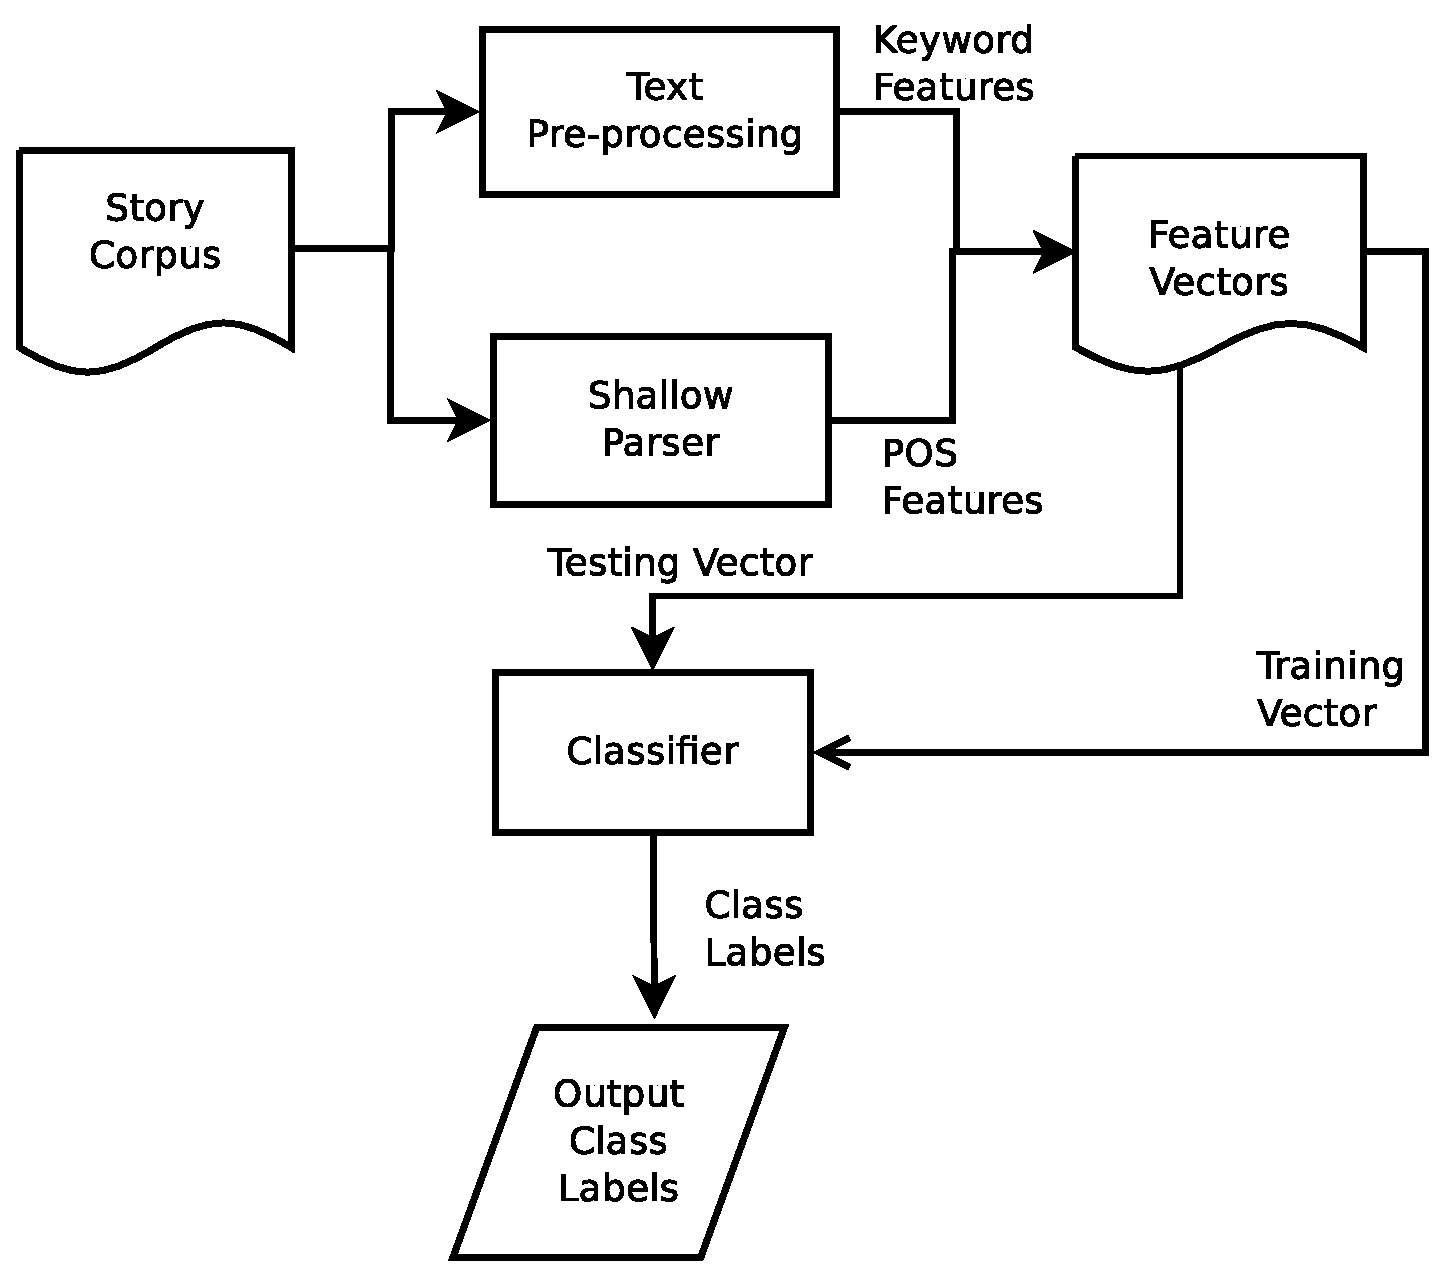
\includegraphics{figures/system}}
\centering
\caption{Flow diagram of Story Classification Framework}
\label{system}
\end{figure}

\newpage

\subsubsection{Database Preparation} \label{Database Preparation}

Hindi and Telugu story corpora consisting of 300 and 150 short stories respectively, are collected from Blogs\footnote{http://telugubalalu.blogspot.in/}, Panchatantra and Akbar-Birbal books. No standard story corpora are available for Indian languages. Details of the Hindi and Telugu story corpora are presented in Table \ref{corpus}. 

\begin{table}[h]
\renewcommand{\arraystretch}{1}
\footnotesize\setlength{\tabcolsep}{8pt}
\caption{Details of Hindi and Telugu Story Corpora\label{corpus}}
\centering
\begin{tabular}{|c|c|c|c|c|}
\hline
\multirow{2}{*}{Story genre} & \multicolumn{2}{c|}{Hindi} & \multicolumn{2}{c|}{Telugu} \\ \cline{2-5} 
 & \# Stories & \# Words & \# Stories & \# Words \\ \hline
Fable & 100 & 50344 & 50 & 6668  \\ \hline
Folk-tale & 100 & 46900 & 50 & 6144  \\ \hline
Legend & 100 & 35991 & 50 & 8540  \\ \hline
\end{tabular}
\end{table}

\subsubsection{Text Pre-processing and POS Tagging} \label{Text Processing and POS Tagging}

Text pre-processing is done to clean the story corpus which includes stripping multiple white spaces, removing special symbols and numbers. Furthermore, Hindi and Telugu shallow parser\footnote{http://ltrc.iiit.ac.in/showfile.php?filename=downloads/shallow\_parser.php} developed by IIIT Hyderabad are used for POS tagging and lemmatization i.e. to convert each word into its root word. No standard stopword lists for Hindi and Telugu are available. In this work, a list of 164 and 138 stopwords respectively, for Hindi and Telugu are prepared and used.

\subsubsection{Feature Extraction} \label{Feature Extraction}

Linguistic-based features such as \textit{POS density (PD)} and Keyword-based features like \textit{Term frequency (TF), Term frequency inverse document frequency (TFIDF)} are explored. Different combinations of POS and keyword-based features are considered for evaluation. All stories in the collection can be regarded as a \textit{document-term matrix (DTM)}, where each row represents a story and each column represents a term in the collection. ``R" statistical programming language is used for feature extraction.


\begin{itemize}
\item[--] \textbf{Term Frequency (TF)}: Frequency of terms in a story are calculated. TF measure explains the importance of a word within a story genre.

\item[--] \textbf{Term Frequency Inverse Document Frequency (TFIDF)}: For a term, weight is assigned as the product of TF and IDF. IDF is calculated as 
\begin{equation*}
idf(t_{i}) = log \frac{N}{n_{i}} 
\end{equation*}

where N is the total number of stories and $n_{i}$ is the number of stories in the corpus that contains word $t_{i}$. TFIDF measure gives importance of a word across story genre.

\item[--] \textbf{POS Density (PD)}: POS tags used here are: Noun (NN), Proper Noun (NNP), Spatial and Temporal Nouns (NST), Pronoun (PRP), Finite Verb (VM), Auxiliary Verb (VAUX), Post Position (PSP), Particles (RP), Adjective (JJ) and Quantifiers (QF). For each document, PD is used as a feature vector. It is calculated as

\begin{equation*}
PD = \sum_{\substack{
   p \in P 
  }}
 \frac{count(p)}{Total\ words\ in\ Document}  \\
 \end{equation*} 
 where P = NN, VM, PRP, VAUX, NNP, NST, PSP, RP, JJ and QF. 

\end{itemize}

\subsubsection{Classifiers}  

Five different combinations of features are explored in this work: PD, TF, TFIDF, TF + PD and TFIDF + PD. The Performance of feature selection methods is evaluated using three classifiers: NB, KNN and SVM. Classifier performance is evaluated using 10-fold cross validation. In this work, we used WEKA as a framework combined with LibSVM package for the implementation of these classifiers.
 

\subsubsection{Evaluation Measures} \label{Evaluation} 

The performance of the classifier is evaluated using \textit{Precision (P), Recall (R), F-measure (F) and Accuracy}. Macro F1 measure is also used as a metric to evaluate the performance. Macro F1 computes a simple average of individual F-measures over classes. McNemar's statistical significance test is used to compare cross-classifier performance. 

%Results are evaluated using Precision (P), Recall (R), F-measure (F) and Accuracy.

\begin{equation*}
P = \frac{No.\ of\ stories\ correctly\ classified\ as\ class\ ``x"}{No.\ of\ stories\ classified\ as\ class\ ``x"} 
\end{equation*}

%R = \frac{Proportion\ classified\ as\ class\ x}{Actual\ classified\ as\ class\ x} 
\begin{equation*}
R = \frac{No.\ of\ stories\ correctly\ classified\ as\ class\ ``x"}{Actual\ No.\ of\ stories\ of\ class\ ``x"} 
\end{equation*}

\begin{equation*}
F = \frac{2\times P\times R}{(P +R)} 
\end{equation*}

\begin{equation*}
Accuracy = \frac{No.\ of\ stories\ correctly\ classified}{Total\ No.\ of\ stories}
\end{equation*}


\begin{equation*}
Macro\ F1 = \frac{\displaystyle\sum_{i \in C} F_i}{\mid C \mid}
\end{equation*}

Where $C$ is the set of predefined classes and $F_i$ is the F-measure for the $i^{th}$ class in $C$. 



\subsection{Story Classification using Keyword based Features} \label{Story Classification using Keyword Features}

For moderate collection of stories, the document-term matrix is likely to have thousands of columns (terms). It is observed that most of the entries in DTM are zeros. For effective representation, we can reduce the dimension of the feature vector using appropriate feature dimension reduction techniques. We have experimented with two feature reduction techniques: (\romannumeral 1) \textit{Sparse Term Removal} and (\romannumeral 2) \textit{Latent Semantic Analysis (LSA)}.
	
	\begin{itemize}

\item[--] \textbf{Sparse Term Removal:} It reduces the higher dimensional document-term matrix to a low dimension matrix by removing the sparse terms. Given a sparsity value, terms having sparseness value more than specified value are removed from document-term matrix. We experimented with different sparseness factors (0.7, 0.75, 0.8, 0.85, 0.9, 0.95)

\item[--] \textbf{Latent Semantic Analysis:} LSA is a method for dimensionality reduction in which original document-term vector space is transformed into a lower dimensional space which captures the behaviour of implicit higher-order structure. LSA is based on the singular value decomposition (SVD) which is commonly used in dimension reduction for document classification. We have experimented with different values of $k$ i.e. (25, 50, 75, 100, 125, 150) and (15, 30, 45, 60, 75, 90) for Hindi and Telugu, respectively. 

\end{itemize}

Tables \ref{Table: Feature Reduction Hindi} and \ref{Table: Feature Reduction Telugu} represent macro F1 measure for story classification using feature reduction techniques for Hindi and Telugu, respectively. Term frequency (TF) is used as a feature to calculate the macro F1 measure. Dimensions of the document-term matrix are listed in the fourth row of the tables. By increasing the sparseness factor, the most frequently repeated terms in story corpora are included in DTM. Increasing the sparseness factor beyond a threshold can add noisy terms, which do not contribute for identifying the story genre and thus decreases the performance. The poor performance of LSA can be attributed to the failure of capturing the behaviour of implicit higher-order structure by lower dimensional document-term matrix. Out of these two feature reduction techniques, the highest F1 measure is achieved using sparseness factor of \textbf{0.9}. 

%analyzing these relations for the story corpora used in this work. 

%document-term vector space is transformed into a lower dimensional space which captures the behaviour of implicit higher-order structure.

%LSA analyzes term-term, term-document, and document-document relationships for feature reduction. But the stories present in our story corpora are closely related to each other like influence of fable can be seen in folk-tale stories and vice versa.



\begin{table}[!htbp] 
\renewcommand{\arraystretch}{1.4}
\caption{Macro F1 measure for story classification using feature reduction techniques for Hindi\label{Table: Feature Reduction Hindi}} 
\resizebox{\linewidth}{!}{
\footnotesize\setlength{\tabcolsep}{0.25pt}
\begin{tabular}{|c||c||c|c|c|c|c|c||c|c|c|c|c|c|}
\hline
\multirow{4}{*}{Classifiers} & \multirow{3}{*}{Full Story} & \multicolumn{12}{c|}{Dimension Reduction Techniques} \\ \cline{3-14} 
 &  & \multicolumn{6}{c||}{Sparseness Factor} & \multicolumn{6}{c|}{LSA} \\ \cline{3-14} 
 &  & 0.7 & 0.75 & 0.8 & 0.85 & 0.9 & 0.95 & 25 & 50 & 75 & 100 & 125 & 150 \\ \cline{2-14} 
 & 300$\times$6608 & 300$\times$78 & 300$\times$104 & 300$\times$143 & 300$\times$182 & 300$\times$366 & 300$\times$681 & 300$\times$25 & 300$\times$50 & 300$\times$75 & 300$\times$100 & 300$\times$125 & 300$\times$150 \\ \hline \hline
NB & 0.71 & 0.81 & 0.83 & 0.84 & 0.86 & \textbf{0.89} & 0.84 & 0.4 & 0.4 & 0.41 & 0.41 & \textbf{0.43} & 0.42 \\ \hline
KNN & 0.61 & 0.71 & 0.73 & 0.74 & 0.75 & \textbf{0.77} & 0.73 & 0.62 & 0.63 & 0.63 & 0.67 & \textbf{0.68} & 0.65 \\ \hline
SVM & 0.62 & 0.79 & 0.82 & 0.85 & 0.86 & \textbf{0.91} & 0.82 & 0.32 & 0.37 & 0.41 & 0.46 & \textbf{0.48} & 0.47 \\ \hline
\end{tabular}}
\end{table}	

\begin{table}[!htbp]
\renewcommand{\arraystretch}{1.4}
\caption{Macro F1 measure for story classification using feature reduction techniques for Telugu\label{Table: Feature Reduction Telugu}} 
\resizebox{\linewidth}{!}{
\footnotesize\setlength{\tabcolsep}{0.25pt}
\begin{tabular}{|c||c||c|c|c|c|c|c||c|c|c|c|c|c|}
\hline
\multirow{4}{*}{Classifiers} & \multirow{3}{*}{Full Story} & \multicolumn{12}{c|}{Dimension Reduction Techniques} \\ \cline{3-14} 
 &  & \multicolumn{6}{c||}{Sparseness Factor} & \multicolumn{6}{c|}{LSA} \\ \cline{3-14} 
  &  & 0.7 & 0.75 & 0.8 & 0.85 & 0.9 & 0.95 & 15 & 30 & 45 & 60 & 75 & 90 \\ \cline{2-14} 
 & 150$\times$4539 & 150$\times$17 & 150$\times$29 & 150$\times$49 & 150$\times$88 & 150$\times$232 & 150$\times$582 & 150$\times$15 & 150$\times$30 & 150$\times$45 & 150$\times$60 & 150$\times$75 & 150$\times$90 \\ \hline \hline
NB & 0.76 & 0.78 & 0.8 & 0.81 & 0.83 & \textbf{0.86} & 0.8 & 0.64 & 0.66 & \textbf{0.67} & 0.61 & 0.56 & 0.54 \\ \hline
KNN & 0.46 & 0.68 & 0.7 & 0.72 & 0.73 & \textbf{0.75} & 0.71 & 0.63 & 0.65 & \textbf{0.71} & 0.63 & 0.58 & 0.46 \\ \hline
SVM & 0.81 & 0.84 & 0.85 & 0.87 & 0.89 & \textbf{0.94} & 0.87 & 0.44 & 0.51 & \textbf{0.58} & 0.56 & 0.55 & 0.52 \\ \hline
\end{tabular}}
\end{table}	

\newpage

\subsection{Story Classification using POS Features}

For analysis, top 10 POS tags in terms of frequency of occurrence are selected. Details of the POS tags selected in this work are presented in Table~\ref{POS Distribution}. For the investigation of the effect of linguistic information on story classification, we carried out experiments with different combinations of POS tags. The POS groups based on syntactic category are listed in Table \ref{Table: POS Sets}. Stories are classified based on these POS tag-sets and macro F1 measures for different POS tag-sets are shown in Table \ref{Table: POS}. Set 2 has the highest macro F1 measure compared to the other POS tag-sets. This result shows the importance of nouns, adjectives and quantifiers for story classification. It is also observed that the performance of POS features are not good as compared to keyword based features. 

		
\begin{table}[!htbp]
\renewcommand{\arraystretch}{1}
\caption{POS distribution across story genres\label{POS Distribution}} 
\footnotesize\setlength{\tabcolsep}{6pt}
\centering
\begin{tabular}{|c|c|c|c||c|c|c|}
\hline
\multirow{2}{*}{POS Tags} & \multicolumn{3}{c||}{Hindi} & \multicolumn{3}{c|}{Telugu} \\ \cline{2-7} 
 & Fable & Folk-tale & Legend & Fable & Folk-tale & Legend \\ \hline
NN & 10975 & 9985 & 7277 & 2539 & 2386 & 2957 \\ \hline
VM & 9298 & 8439 & 6098 & 1919 & 1730 & 2377 \\ \hline
PSP & 6788 & 6249 & 4898 & 104 & 110 & 131 \\ \hline
PRP & 5286 & 4910 & 3761 & 615 & 557 & 769 \\ \hline
VAUX & 4278 & 3735 & 2817 & 40 & 38 & 48 \\ \hline
JJ & 1691 & 1698 & 1420 & 264 & 217 & 238 \\ \hline
NNP & 1534 & 1497 & 1554 & 22 & 152 & 516 \\ \hline
RP & 1456 & 1353 & 1011 & 45 & 38 & 86 \\ \hline
NST & 1035 & 764 & 584 & 275 & 178 & 283 \\ \hline
QF & 635 & 530 & 503 & 61 & 40 & 75 \\ \hline
\end{tabular}
\end{table}

 
\begin{table}[h]
\renewcommand{\arraystretch}{0.9}
\caption{Different sets of POS tags\label{Table: POS Sets}} 
\centering
\begin{tabular}{|c|c|}
\hline
Set & POS Tags\\
\hline
Set 1 & $\lbrace NN, NNP, NST, PRP, JJ, QF, VM, VAUX, PSP, RP \rbrace$ \\ \hline
Set 2 & $\lbrace NN, NNP, NST, PRP, JJ, QF \rbrace$\\ \hline
Set 3 & $\lbrace NN, NNP, NST, PRP, VM, VAUX \rbrace$ \\ \hline
Set 4 & $\lbrace NN, NNP, NST, PRP, PSP, RP \rbrace$\\ \hline
Set 5 & $\lbrace NN, NNP, NST, PRP \rbrace$\\ \hline
Set 6 & $\lbrace JJ, QF, VM, VAUX \rbrace$\\
 \hline
\end{tabular}
\end{table}
	

\begin{table}[!htbp]
\renewcommand{\arraystretch}{0.9}
\caption {Macro F1 measures for different sets of POS tags \label{Table: POS}}
\footnotesize\setlength{\tabcolsep}{6pt}
\centering
\begin{tabular}{|c|c|c|c||c|c|c|}
\hline
\multirow{2}{*}{Set} & \multicolumn{3}{c||}{Hindi} & \multicolumn{3}{c|}{Telugu} \\ \cline{2-7} 
 & NB & KNN & SVM & NB & KNN & SVM \\ \hline
Set 1 & 0.48 & 0.4 & 0.45 & 0.55 & 0.47 & 0.56 \\ \hline
Set 2 & \textbf{0.49} & \textbf{0.43} & \textbf{0.5} & \textbf{0.56} & \textbf{0.55} & \textbf{0.58} \\ \hline
Set 3 & 0.48 & 0.4 & 0.48 & 0.55 & 0.51 & 0.57 \\ \hline
Set 4 & 0.48 & 0.38 & 0.47 & 0.54 & 0.52 & 0.56 \\ \hline
Set 5 & 0.45 & 0.4 & 0.46 & 0.53 & 0.51 & 0.56 \\ \hline
Set 6 & 0.42 & 0.33 & 0.39 & 0.38 & 0.38 & 0.36 \\ \hline
\end{tabular}
\end{table}

\newpage

\subsection{Story Classification using Concatenation of Keyword and POS Features}

	A detailed performance measures for story classification using the concatenation of keyword and POS features is given in Table \ref{Table: Story Classifiation Performance After Modification}. PD feature corresponds to POS density of Set 2 POS tags (See Table \ref{Table: POS Sets}). Story classification accuracy using keyword and POS features is shown in Figure \ref{Figure: Story Accuracy set 2}. Tables  \ref{Table: Mcnemar result of significance test} and \ref{Table: Cross classifier significance test} summarizes the McNemar's statistical significance test results for different combinations of features and cross-classifier performance respectively. The meaning of symbols used in the Tables \ref{Table: Mcnemar result of significance test} and \ref{Table: Cross classifier significance test} are as follows: (\romannumeral 1) `` $\gg$ " means \textit{P-value} $\leq$ 0.01, which is extremely statistically significant, (\romannumeral 2) `` $>$ " means 0.01 $<$ \textit{P-value} $\leq$ 0.05, which is statistically significant and (\romannumeral 3) `` $\sim$ " means \textit{P-value} $>$ 0.05, which is not statistically significant. From the tables, it is evident that adding PD features to TF and TFIDF improves the F-measure slightly. Among the three classifiers explored in this work, the performance of SVM is better than NB and KNN in terms of F-measure for both Hindi and Telugu stories. 
	
	The Keyword and POS features are based on terms (words) present in a story. Moreover, while analyzing the story corpora, it is noted that some of the terms are common for both fable and folk-tale. The terms in legend story are easily distinguishable from fable and folk-tale. NB is a probabilistic learning method. It is based on Bayes theorem and the story genre will be assigned to the class having \textit{maximum a posteriori probability}. KNN classifies the story based on the similarities between features i.e terms used in story. The poor performance of KNN can be due to the noisy terms in the stories. SVM performs classification by constructing hyperplane in a high dimensional space that maximizes the margin between classes. SVM is resilient to noise because the classifier performance depends on the support vectors. Hence SVM has the best accuracy. 


%KNN classifies the story based on the similarities between story genres. The stories present in our story corpora are closely related to each other like influence of fable can be seen in folk-tale stories and vice versa. This may be the reason for low performance of KNN. 

	
	\begin{table}[!htbp]
\renewcommand{\arraystretch}{1.3}
\caption {Performance measures for story classificaiton using concatenation of keyword and POS features \label{Table: Story Classifiation Performance After Modification}}
\resizebox{\linewidth}{!}{
\footnotesize\setlength{\tabcolsep}{2pt}
\begin{tabular}{|c|c|c|c|c|c|c|c|c|c|c||c|c|c|c|c|c|c|c|c|}
\hline
\multirow{3}{*}{Story Genre} & \multirow{3}{*}{Features} & \multicolumn{9}{c||}{Hindi} & \multicolumn{9}{c|}{Telugu} \\ \cline{3-20} 
 &  & \multicolumn{3}{c|}{NB} & \multicolumn{3}{c|}{KNN} & \multicolumn{3}{c||}{SVM} & \multicolumn{3}{c|}{NB} & \multicolumn{3}{c|}{KNN} & \multicolumn{3}{c|}{SVM} \\ \cline{3-20} 
 &  & P & R & F & P & R & F & P & R & F & P & R & F & P & R & F & P & R & F \\ \hline
\multirow{5}{*}{Fable} & PD & 0.46 & 0.65 & 0.54 & 0.47 & 0.70 & 0.57 & 0.46 & 0.48 & 0.48 & 0.56 & 0.62 & 0.59 & 0.48 & 0.72 & 0.58 & 0.59 & 0.96 & 0.73 \\ \cline{2-20} 
 & TF & 0.93 & 0.88 & 0.9 & 0.89 & 0.59 & 0.71 & 0.94 & 0.91 & 0.92 & 0.95 & 0.8 & 0.87 & 0.68 & 0.7 & 0.69 & 0.94 & 0.94 & 0.94 \\ \cline{2-20} 
  & TF + PD & 0.93 & 0.90 & \textbf{0.91} & 0.89 & 0.68 & \textbf{0.77} & 0.95 & 0.93 & \textbf{0.94} & 0.98 & 0.82 & \textbf{0.89} & 0.78 & 0.76 & \textbf{0.77} & 0.98 & 0.96 & \textbf{0.97} \\ \cline{2-20} 
 & TFIDF & 0.89 & 0.44 & 0.59 & 0.86 & 0.56 & 0.68 & 0.92 & 0.9 & 0.91 & 0.86 & 0.74 & 0.8 & 0.64 & 0.64 & 0.64 & 0.92 & 0.92 & 0.92 \\ \cline{2-20} 
 & TFIDF + PD & 0.9 & 0.75 & \textbf{0.81} & 0.88 & 0.66 & \textbf{0.75} & 0.94 & 0.92 & \textbf{0.93} & 0.93 & 0.78 & \textbf{0.85} & 0.72 & 0.68 & \textbf{0.7} & 0.94 & 0.92 & \textbf{0.93} \\ \hline
\multirow{5}{*}{Folk-tale} & PD & 0.63 & 0.35 & 0.45 & 0.38 & 0.31 & 0.34 & 0.52 & 0.41 & 0.46 & 0.46 & 0.72 & 0.56 & 0.55 & 0.30 & 0.39 & 0.58 & 0.22 & 0.32 \\ \cline{2-20} 
 & TF & 0.87 & 0.87 & 0.87 & 0.66 & 0.84 & 0.74 & 0.96 & 0.9 & 0.93 & 0.75 & 0.92 & 0.83 & 0.86 & 0.76 & 0.8 & 0.96 & 0.92 & 0.94 \\ \cline{2-20} 
 & TF + PD & 0.87 & 0.90 & \textbf{0.89} & 0.75 & 0.86 & \textbf{0.8} & 0.97 & 0.92 & \textbf{0.94} & 0.76 & 0.94 & \textbf{0.84} & 0.8 & 0.82 & \textbf{0.81} & 0.98 & 0.94 & \textbf{0.96} \\ \cline{2-20}
 & TFIDF & 0.76 & 0.76 & 0.76 & 0.65 & 0.82 & 0.73 & 0.94 & 0.89 & 0.91 & 0.74 & 0.84 & 0.78 & 0.78 & 0.72 & 0.75 & 0.94 & 0.9 & 0.92 \\ \cline{2-20} 
 & TFIDF + PD & 0.82 & 0.8 & \textbf{0.81} & 0.7 & 0.83 & \textbf{0.76} & 0.94 & 0.9 & \textbf{0.92} & 0.79 & 0.86 & \textbf{0.82} & 0.76 & 0.78 & \textbf{0.77} & 0.96 & 0.92 & \textbf{0.94} \\ \hline
\multirow{5}{*}{Legend} & PD & 0.59 & 0.39 & 0.47 & 0.49 & 0.34 & 0.40 & 0.54 & 0.54 & 0.54 & 0.87 & 0.40 & 0.55 & 0.75 & 0.60 & 0.67 & 0.72 & 0.62 & 0.67 \\ \cline{2-20} 
 & TF & 0.87 & 0.93 & 0.9 & 0.85 & 0.9 & 0.87 & 0.85 & 0.94 & 0.89 & 0.91 & 0.86 & 0.88 & 0.72 & 0.8 & 0.76 & 0.92 & 0.96 & 0.93 \\ \cline{2-20} 
 & TF + PD & 0.96 & 0.96 & \textbf{0.96} & 0.84 & 0.92 & \textbf{0.88} & 0.9 & 0.96 & \textbf{0.93} & 0.96 & 0.88 & \textbf{0.92} & 0.84 & 0.84 & \textbf{0.84} & 0.92 & 0.98 & \textbf{0.95} \\ \cline{2-20} 
 & TFIDF & 0.64 & 0.96 & 0.77 & 0.82 & 0.9 & 0.86 & 0.86 & 0.92 & 0.88 & 0.82 & 0.82 & 0.82 & 0.68 & 0.74 & 0.71 & 0.9 & 0.94 & 0.91 \\ \cline{2-20} 
 & TFIDF + PD & 0.74 & 0.88 & \textbf{0.8} & 0.84 & 0.91 & \textbf{0.87} & 0.87 & 0.93 & \textbf{0.9} & 0.81 & 0.88 & \textbf{0.84} & 0.77 & 0.8 & \textbf{0.78} & 0.9 & 0.96 & \textbf{0.93} \\ \hline
 \end{tabular}}
\end{table}


\begin{figure}[!htbp] 
\centering
%\resizebox{16cm}{7cm}{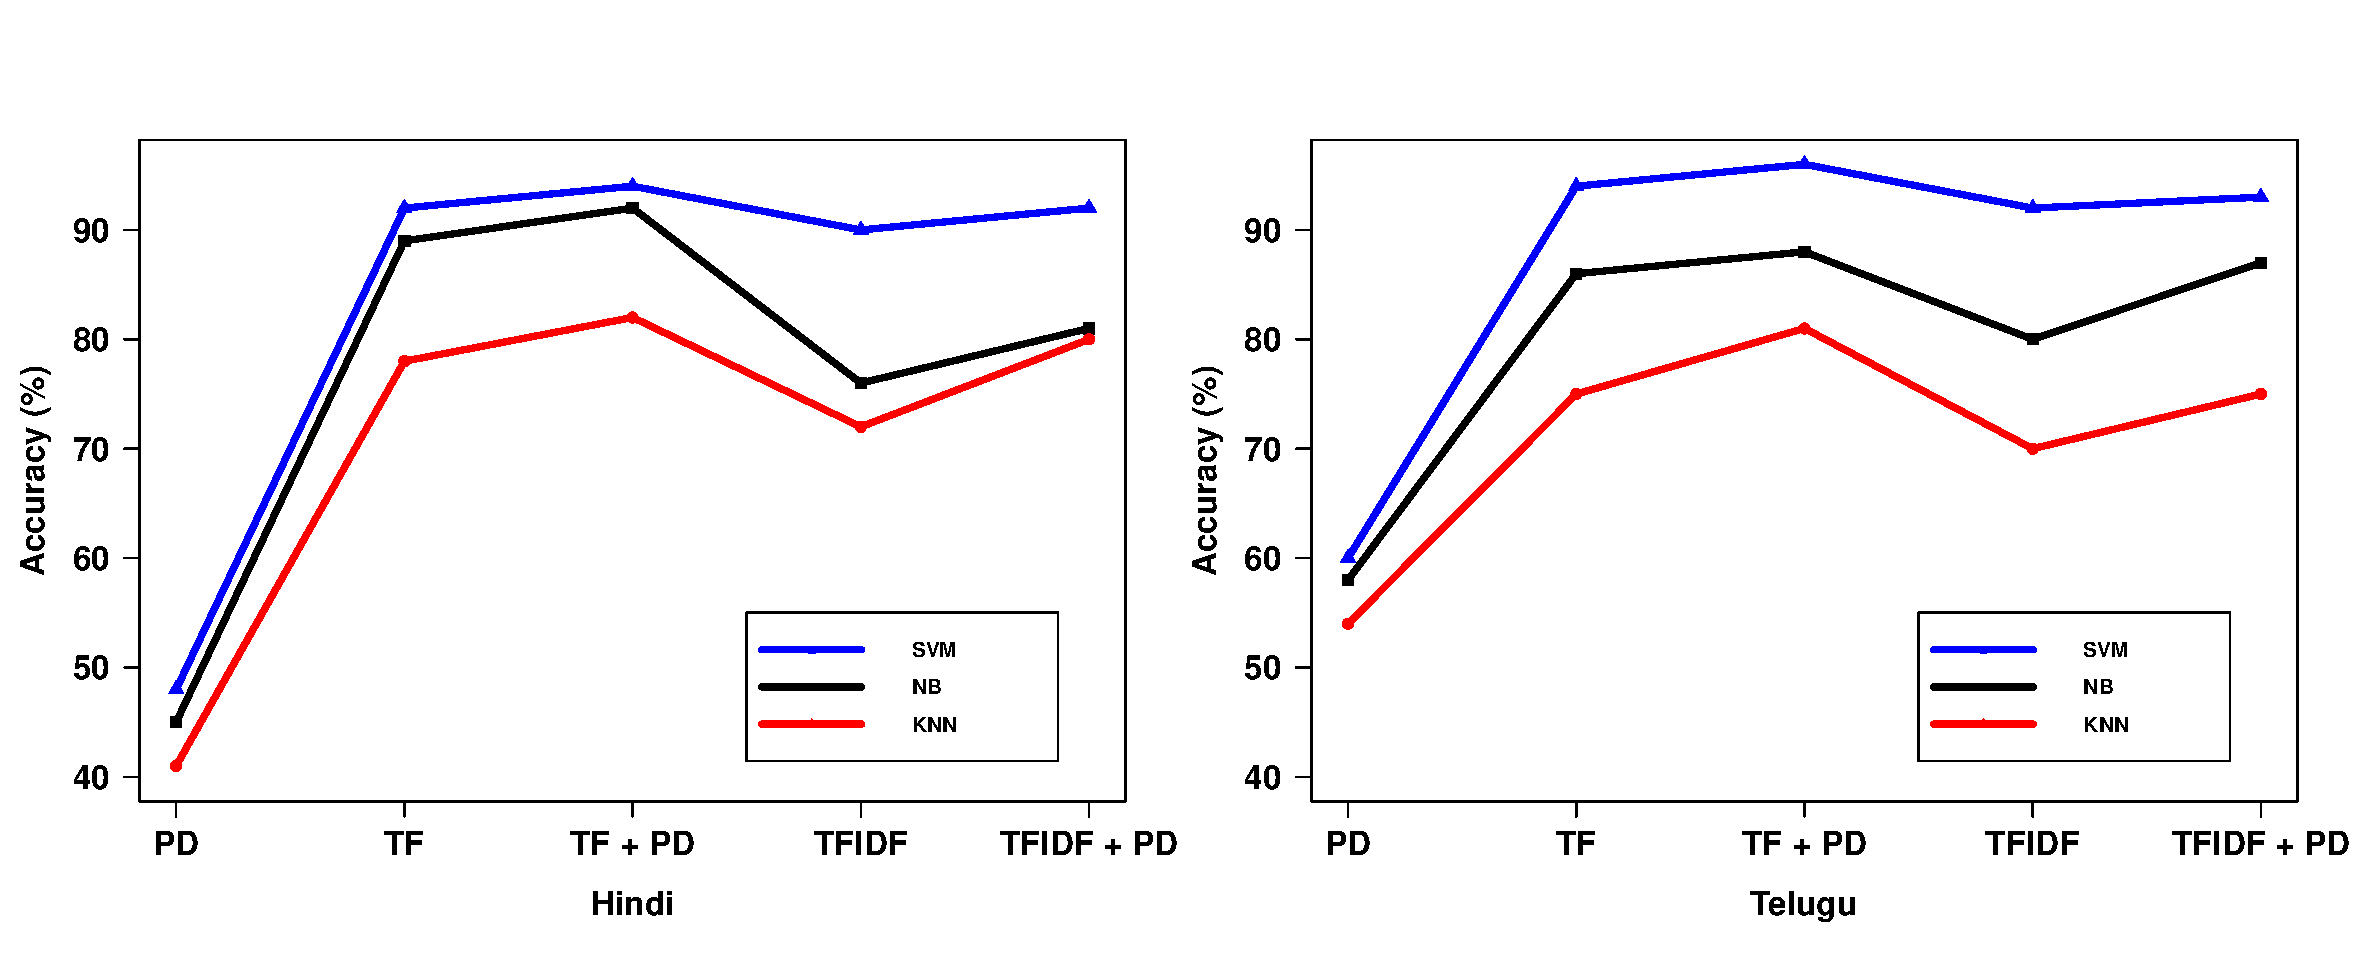
\includegraphics{figures/Story_Cln_90_set_2}}
\resizebox{16cm}{7cm}{\includegraphics{figures/Story_Cln_bw_90_set_2}}
\centering
\caption{Story classification accuracy using concatenation of keyword and POS features}
\label{Figure: Story Accuracy set 2}
\end{figure}	


\begin{table}[!htbp]
\renewcommand{\arraystretch}{1.2}
\caption {Statistical significance test results for different combination of features \label{Table: Mcnemar result of significance test}}
\footnotesize\setlength{\tabcolsep}{2pt}
\centering
\begin{tabular}{|c|c|c||c|c|}
\hline
\multirow{2}{*}{Classifier} & \multicolumn{2}{c||}{Hindi} & \multicolumn{2}{c|}{Telugu} \\ \cline{2-5} 
 & TF + PD vs TF & TFIDF + PD vs TFIDF & TF + PD vs TF & TFIDF + PD vs TFIDF \\ \hline
NB & $>$ & $\sim$ & $>$ & $\sim$ \\ \hline
KNN & $\sim$ & $\sim$ & $\sim$ & $\sim$ \\ \hline
SVM & $>$ & $>$ & $>$ & $>$ \\ \hline
\end{tabular}
\end{table}	
	
\begin{table}[!htbp]
\renewcommand{\arraystretch}{1.2}
\caption{Statistical significance test results for cross-classifier performance \label{Table: Cross classifier significance test}}
\resizebox{\linewidth}{!}{
\footnotesize\setlength{\tabcolsep}{2pt}
\centering
\begin{tabular}{|c|c|c|c|c|c|c||c|c|c|c|c|}
\hline
\multirow{2}{*}{Classifier A} & \multirow{2}{*}{Classifier B} & \multicolumn{5}{c||}{Hindi} & \multicolumn{5}{c|}{Telugu} \\ \cline{3-12} 
 &  & PD & TF & TF + PD & TFIDF & TFIDF + PD & PD & TF & TF + PD & TFIDF & TFIDF + PD \\ \hline
NB & KNN & $\sim$ & $\gg$ & $\gg$ & $>$ & $\sim$ & $\sim$ & $\gg$ & $\gg$ & $\gg$ & $\gg$ \\ \hline
SVM & KNN & $\sim$ & $\gg$ & $\gg$ & $\gg$ & $\gg$ & $\sim$ & $\gg$ & $\gg$ & $\gg$ & $\gg$ \\ \hline
SVM & NB & $\sim$ & $\sim$ & $\sim$ & $\gg$ & $\gg$ & $\sim$ & $\gg$ & $>$ & $\gg$ & $>$ \\ \hline
\end{tabular}}
\end{table} 


	
\section{Summary and Conclusion}

In this work, Hindi and Telugu children stories are classified into three genres: fable, folk-tale and legend. The significant contributions of this work are: (\romannumeral 1) story classification using keyword based features, (\romannumeral 2) story classification using POS features and (\romannumeral 3) story classification using concatenation of keyword and POS features. Hindi and Telugu story corpora consisting of 300 and 150 short stories are used for experimentation. NB, KNN and SVM classifiers are used to evaluate the story classification performance using 10-fold cross validation. The effectiveness of classifiers is measured using Precision, Recall and F-measure. McNemar's statistical significance test are conducted to compare cross-classifier performance. Results showed that using linguistic information boosts the performance of story classification significantly. From the experiments conducted on the analysis of POS tags, it is observed that POS tag set consisting of nouns, adjectives and quantifiers have the highest accuracy compared to the other tag sets. In most of the cases, the highest performance is achieved by TF + PD features and SVM models outperformed the other models in terms of classification accuracy. 



\section{Future Work}

\begin{enumerate}
\item \textit{Story classification using partial story information:} Exploring story classification by dividing stories into parts based on story semantics and also to find the optimal number of sentences required to identify story genres.
\item \textit{Emotion prediction from story text:} Exploring Keyword, POS and story specific features for predicting emotion from story text. \\ 
\item \textit{Deriving prosody rules:} Deriving prosody rules (modification factors) specific to emotions and story genres. The prosody modification factors can be derived carefully by analyzing the perceptual differences between synthesized neutral speech utterances and their respective utterances narrated by a storyteller. 
\item \textit{Synthesis of story speech using mark-up language:} Story-specific prosody rules can be effectively incorporated using SABLE mark-up language. The quality and naturalness of the synthesized story speech can be evaluated using subjective tests.
\end{enumerate}


\section*{Publications} 
\begin{itemize}
		\item[] { \bf {Conference:}}
	\begin{enumerate}
	 	\item \textbf{Harikrishna D M} and K. Sreenivasa Rao, ``Classification of Children Stories in Hindi Using Keywords and POS Density," in \textit{International Conference on Computer Communication and Control (IC4)}, Indore, 2015.
	 	\end{enumerate}
	 	\end{itemize}
	 


\section*{Acknowledgements}
We are thankful to the Department of Information Technology, Govt. of India for supporting this research work, \textit{Development of Text-to-Speech synthesis for Indian Languages Phase II}, Ref. no. 11(7)/2011HCC(TDIL)


\bibliographystyle{plain}
\bibliography{Ref}
\end{document}	
	
	
	
	



%\subsection{Story Classification Based on Story Parts} \label{Story classification based on Structure}
%	
%	In this section, we tried to explore the embedded story genre information by dividing the story into parts. In this work, stories are (\romannumeral 1) manually divided into parts based on story semantics as \textit{introduction, main and climax}; and (\romannumeral 2) automatically divided into equal parts as \textit{initial, middle and end}. Details of story corpora based on parts are shown in Table \ref{Table: Story Corpus Sentences Stats}. 
%	
%\begin{table}[h]
%\renewcommand{\arraystretch}{1}
%\caption{Statistical Information of Hindi and Telugu story corpora based on number of sentences \label{Table: Story Corpus Sentences Stats}}
%\footnotesize\setlength{\tabcolsep}{2pt}
%\centering
%\begin{tabular}{|c|c|c|c||c|c|c||c|c|c|}
%\hline
%\multirow{2}{*}{Story Corpus} & \multirow{2}{*}{\# Stories} & \multirow{2}{*}{\# Sentences} & \multicolumn{7}{c|}{Average \# of Sentences} \\ \cline{4-10} 
% &  &  & Full Story & Introduction & Main & Climax & Initial & Middle & End \\ \hline
%Hindi & 300 & 7520 & 25 & 4 & 13 & 7 & 7 & 8 & 8 \\ \hline
%Telugu & 150 & 2720 & 18 & 3 & 9 & 5 & 5 & 6 & 6 \\ \hline
%\end{tabular}
%\end{table}
%
%	
%	
%Based on story semantics, a children story can be divided into three parts as: introduction, main and climax. Introduction part comprises of introducing characters that are involved in the rest of story. Main part constitutes the core component of the story. The conclusion of the story along with moral are described in the climax part. In this work, entire stories are manually divided into three parts and to avoid any annotation bias we took inter-annotator agreement. Fleiss Kappa ($\kappa$) is a statistical measure of inter-annotator agreement and $\kappa = 0.774$ and $0.76$ are observed from the annotation of Hindi and Telugu respectively which are considered to be substantial agreement. Table \ref{Table: Story by parts based on context Macro F1} represents the Macro F1 measure for story classification by parts based on the story semantics. Baseline corresponds to the TF features for the individual part of stories without lemmatization and stopword removal. PD corresponds to POS density of $\lbrace NN, NNP, NST, PRP, JJ, QF \rbrace$ tags.
%
%\begin{table}[h]
%\renewcommand{\arraystretch}{1}
%\caption{Macro F1 measure for story by parts based on introduction, main and climax parts of the story \label{Table: Story by parts based on context Macro F1}}
%\footnotesize\setlength{\tabcolsep}{1pt}
%\centering
%\begin{tabular}{|c|c|c|c|c|c|c||c|c|c|c|c|c||c|c|c|c|c|c|}
%\hline
%\multirow{3}{*}{Features} & \multicolumn{6}{c||}{Introduction} & \multicolumn{6}{c||}{Main} & \multicolumn{6}{c|}{Climax} \\ \cline{2-19} 
% & \multicolumn{3}{c|}{Hindi} & \multicolumn{3}{c||}{Telugu} & \multicolumn{3}{c|}{Hindi} & \multicolumn{3}{c||}{Telugu} & \multicolumn{3}{c|}{Hindi} & \multicolumn{3}{c|}{Telugu} \\ \cline{2-19} 
% & NB & KNN & SVM & NB & KNN & SVM & NB & KNN & SVM & NB & KNN & SVM & NB & KNN & SVM & NB & KNN & SVM \\ \hline
%Baseline & 0.55 & 0.42 & 0.57 & 0.56 & 0.41 & 0.6 & 0.59 & 0.44 & 0.63 & 0.6 & 0.42 & 0.62 &  0.46 & 0.41 & 0.53 & 0.5 & 0.4 & 0.59 \\ \hline
%PD & 0.48 & 0.41 & 0.46 & 0.46 & 0.41 & 0.42 & 0.43 & 0.39 & 0.42 & 0.5 & 0.4 & 0.46 & 0.43 & 0.38 & 0.42 & 0.47 & 0.38 & 0.45 \\ \hline
%TF & 0.7 & 0.47 & 0.78 & 0.68 & 0.53 & 0.72 & 0.71 & 0.53 & 0.79 & 0.7 & 0.58 & 0.75 & 0.66 & 0.45 & 0.74 & 0.66 & 0.45 & 0.7 \\ \hline
%TF + PD & 0.72 & 0.54 & \textbf{0.79} & 0.73 & 0.55 & \textbf{0.76} & 0.78 & 0.61 & \textbf{\textit{0.82}} & 0.75 & 0.59 & \textbf{\textit{0.79}} & 0.68 & 0.51 & \textbf{0.75} & 0.71 & 0.46 & \textbf{0.73} \\ \hline
%TFIDF & 0.61 & 0.46 & 0.66 & 0.63 & 0.51 & 0.57 & 0.67 & 0.47 & 0.69 & 0.65 & 0.54 & 0.64 & 0.59 & 0.44 & 0.63 & 0.61 & 0.42 & 0.61 \\ \hline
%TFIDF + PD & 0.64 & 0.47 & 0.67 & 0.64 & 0.52 & 0.62 & 0.69 & 0.48 & 0.7 & 0.66 & 0.56 & 0.66 & 0.6 & 0.44 & 0.64 & 0.62 & 0.44 & 0.63 \\ \hline
%\end{tabular}
%\end{table}
%
% The major drawback of dividing story based on story semantics is that only native speakers or person who knows the particular language can identify the introduction, main and climax parts in a story. To overcome this drawback, we automatically divided stories equally into three parts as: initial, middle and end. Table \ref{Table: Story by parts based on progress Macro F1} represents the Macro F1 measure for story classification based on initial, middle and end parts of the story. Baseline and PD features are similar to the one explained above. 
%
%\begin{table}[h]
%\renewcommand{\arraystretch}{1}
%\caption{Macro F1 measure for story by parts based on initial, middle and end parts of the story \label{Table: Story by parts based on progress Macro F1}}
%\footnotesize\setlength{\tabcolsep}{1pt}
%\centering
%\begin{tabular}{|c|c|c|c|c|c|c||c|c|c|c|c|c||c|c|c|c|c|c|}
%\hline
%\multirow{3}{*}{Features} & \multicolumn{6}{c||}{Initial} & \multicolumn{6}{c||}{Middle} & \multicolumn{6}{c|}{End} \\ \cline{2-19} 
% & \multicolumn{3}{c|}{Hindi} & \multicolumn{3}{c||}{Telugu} & \multicolumn{3}{c|}{Hindi} & \multicolumn{3}{c||}{Telugu} & \multicolumn{3}{c|}{Hindi} & \multicolumn{3}{c|}{Telugu} \\ \cline{2-19}
% & NB & KNN & SVM & NB & KNN & SVM & NB & KNN & SVM & NB & KNN & SVM & NB & KNN & SVM & NB & KNN & SVM \\ \hline
%Baseline & 0.62 & 0.4 & 0.65 & 0.56 & 0.4 & 0.66 & 0.51 & 0.46 & 0.56 & 0.53 & 0.4 & 0.61 & 0.49 & 0.44 & 0.54 & 0.48 & 0.43 & 0.52 \\ \hline
%PD & 0.5 & 0.42 & 0.46 & 0.5 & 0.41 & 0.42 & 0.43 & 0.36 & 0.41 & 0.52 & 0.48 & 0.5 & 0.49 & 0.39 & 0.44 & 0.53 & 0.46 & 0.48 \\ \hline
%TF & 0.75 & 0.5 & 0.79 & 0.68 & 0.39 & 0.74 & 0.68 & 0.49 & 0.76 & 0.68 & 0.44 & 0.73 & 0.58 & 0.47 & 0.7 & 0.66 & 0.5 & 0.7 \\ \hline
%TF + PD & 0.76 & 0.53 & \textbf{\textit{0.8}} & 0.71 & 0.48 & \textbf{\textit{0.76}} & 0.74 & 0.51 & \textbf{0.79} & 0.7 & 0.46 & \textbf{0.75} & 0.59 & 0.49 & \textbf{0.72} & 0.68 & 0.52 & \textbf{0.72} \\ \hline
%TFIDF & 0.66 & 0.45 & 0.67 & 0.62 & 0.42 & 0.63 & 0.54 & 0.51 & 0.64 & 0.6 & 0.41 & 0.62 & 0.59 & 0.48 & 0.61 & 0.62 & 0.47 & 0.55 \\ \hline
%TFIDF + PD & 0.68 & 0.46 & 0.69 & 0.63 & 0.46 & 0.65 & 0.56 & 0.57 & 0.66 & 0.63 & 0.45 & 0.65 & 0.6 & 0.49 & 0.62 & 0.63 & 0.5 & 0.59 \\ \hline
%\end{tabular}
%\end{table}
%
%%% tiil here 
%
% Summarizing the results obtained from the experiments conducted on story classification based on individual parts of the story, it can be concluded that: (\romannumeral 1) $Main$ part of the story is sufficient for better identification of story genres; (\romannumeral 2) $Initial$ part is also has comparatively better performance in story genre identification; (\romannumeral 3) Except for the models built using PD features, $SVM$ outperforms $NB$ and $KNN$ in classification accuracy. Baseline performance is less comparative to the rest of features which is evident that lemmatization and stopword removal boosts the performance of story classification.






%	\subsection{Story Classification Using Sentence Increment Model} \label{Sentence Increment Model}
%	
%	 In this section, we are exploring story classification using sentence increment model. We carried out this experiment: (\romannumeral 1) to check whether there exists any correlation between number of sentences and story structure like introduction, main, initial or middle; (\romannumeral 2) to find the optimum number of sentences required to identify story genres. Sentence increment model aims at building the models by selecting sentences incrementally in the story. For our analysis, we have used first ten sentences and TF feature for model building. 
%	
%	Table \ref{Table: Sentence Increment Performance} shows the macro F1 measures for sentence increment model. For the story corpora used in this work, the initial nine and seven sentences in Hindi and Telugu stories respectively are sufficient for better identification of story genres. 
%	 	
%	\begin{table}[h]
%\renewcommand{\arraystretch}{1}
%\caption{Macro F1 measure for  Performance measure for sentence increment model \label{Table: Sentence Increment Performance}} 
%\footnotesize\setlength{\tabcolsep}{6pt}
%\centering
%\begin{tabular}{|c|c|c|c||c|c|c|}
%\hline
%\multirow{2}{*}{\# of Sentences} & \multicolumn{3}{c||}{Hindi} & \multicolumn{3}{c|}{Telugu} \\ \cline{2-7} 
% & NB & KNN & SVM & NB & KNN & SVM \\ \hline
%1 & 0.7 & 0.51 & 0.75 & 0.65 & 0.4 & 0.68 \\ \hline
%2 & 0.7 & 0.52 & 0.76 & 0.65 & 0.42 & 0.7 \\ \hline
%3 & 0.71 & 0.52 & 0.77 & 0.67 & 0.44 & 0.7 \\ \hline
%4 & 0.72 & 0.53 & 0.77 & 0.7 & 0.46 & 0.72 \\ \hline
%5 & 0.74 & 0.54 & 0.78 & 0.7 & 0.49 & 0.75 \\ \hline
%6 & 0.74 & 0.55 & 0.79 & 0.71 & 0.51 & 0.77 \\ \hline
%7 & 0.76 & 0.56 & 0.8 & \textbf{0.73} & \textbf{0.55} & \textbf{0.79} \\ \hline
%8 & 0.77 & 0.56 & 0.83 & 0.7 & 0.52 & 0.77 \\ \hline
%9 & \textbf{0.79} & \textbf{0.6} & \textbf{0.86} & 0.68 & 0.5 & 0.76 \\ \hline
%10 & 0.77 & 0.57 & 0.82 & 0.68 & 0.49 & 0.75 \\ \hline
%\end{tabular}
%\end{table}



% end of file template.tex

